% Options for packages loaded elsewhere
\PassOptionsToPackage{unicode}{hyperref}
\PassOptionsToPackage{hyphens}{url}
\PassOptionsToPackage{dvipsnames,svgnames,x11names}{xcolor}
%
\documentclass[
  letterpaper,
  DIV=11,
  numbers=noendperiod]{scrreprt}

\usepackage{amsmath,amssymb}
\usepackage{iftex}
\ifPDFTeX
  \usepackage[T1]{fontenc}
  \usepackage[utf8]{inputenc}
  \usepackage{textcomp} % provide euro and other symbols
\else % if luatex or xetex
  \usepackage{unicode-math}
  \defaultfontfeatures{Scale=MatchLowercase}
  \defaultfontfeatures[\rmfamily]{Ligatures=TeX,Scale=1}
\fi
\usepackage{lmodern}
\ifPDFTeX\else  
    % xetex/luatex font selection
\fi
% Use upquote if available, for straight quotes in verbatim environments
\IfFileExists{upquote.sty}{\usepackage{upquote}}{}
\IfFileExists{microtype.sty}{% use microtype if available
  \usepackage[]{microtype}
  \UseMicrotypeSet[protrusion]{basicmath} % disable protrusion for tt fonts
}{}
\makeatletter
\@ifundefined{KOMAClassName}{% if non-KOMA class
  \IfFileExists{parskip.sty}{%
    \usepackage{parskip}
  }{% else
    \setlength{\parindent}{0pt}
    \setlength{\parskip}{6pt plus 2pt minus 1pt}}
}{% if KOMA class
  \KOMAoptions{parskip=half}}
\makeatother
\usepackage{xcolor}
\setlength{\emergencystretch}{3em} % prevent overfull lines
\setcounter{secnumdepth}{5}
% Make \paragraph and \subparagraph free-standing
\ifx\paragraph\undefined\else
  \let\oldparagraph\paragraph
  \renewcommand{\paragraph}[1]{\oldparagraph{#1}\mbox{}}
\fi
\ifx\subparagraph\undefined\else
  \let\oldsubparagraph\subparagraph
  \renewcommand{\subparagraph}[1]{\oldsubparagraph{#1}\mbox{}}
\fi


\providecommand{\tightlist}{%
  \setlength{\itemsep}{0pt}\setlength{\parskip}{0pt}}\usepackage{longtable,booktabs,array}
\usepackage{calc} % for calculating minipage widths
% Correct order of tables after \paragraph or \subparagraph
\usepackage{etoolbox}
\makeatletter
\patchcmd\longtable{\par}{\if@noskipsec\mbox{}\fi\par}{}{}
\makeatother
% Allow footnotes in longtable head/foot
\IfFileExists{footnotehyper.sty}{\usepackage{footnotehyper}}{\usepackage{footnote}}
\makesavenoteenv{longtable}
\usepackage{graphicx}
\makeatletter
\def\maxwidth{\ifdim\Gin@nat@width>\linewidth\linewidth\else\Gin@nat@width\fi}
\def\maxheight{\ifdim\Gin@nat@height>\textheight\textheight\else\Gin@nat@height\fi}
\makeatother
% Scale images if necessary, so that they will not overflow the page
% margins by default, and it is still possible to overwrite the defaults
% using explicit options in \includegraphics[width, height, ...]{}
\setkeys{Gin}{width=\maxwidth,height=\maxheight,keepaspectratio}
% Set default figure placement to htbp
\makeatletter
\def\fps@figure{htbp}
\makeatother

\KOMAoption{captions}{tableheading}
\makeatletter
\@ifpackageloaded{bookmark}{}{\usepackage{bookmark}}
\makeatother
\makeatletter
\@ifpackageloaded{caption}{}{\usepackage{caption}}
\AtBeginDocument{%
\ifdefined\contentsname
  \renewcommand*\contentsname{Indholdsfortegnelse}
\else
  \newcommand\contentsname{Indholdsfortegnelse}
\fi
\ifdefined\listfigurename
  \renewcommand*\listfigurename{Figuroversigt}
\else
  \newcommand\listfigurename{Figuroversigt}
\fi
\ifdefined\listtablename
  \renewcommand*\listtablename{Tabeloversigt}
\else
  \newcommand\listtablename{Tabeloversigt}
\fi
\ifdefined\figurename
  \renewcommand*\figurename{Figur}
\else
  \newcommand\figurename{Figur}
\fi
\ifdefined\tablename
  \renewcommand*\tablename{Tabel}
\else
  \newcommand\tablename{Tabel}
\fi
}
\@ifpackageloaded{float}{}{\usepackage{float}}
\floatstyle{ruled}
\@ifundefined{c@chapter}{\newfloat{codelisting}{h}{lop}}{\newfloat{codelisting}{h}{lop}[chapter]}
\floatname{codelisting}{Liste}
\newcommand*\listoflistings{\listof{codelisting}{Listeoversigt}}
\makeatother
\makeatletter
\makeatother
\makeatletter
\@ifpackageloaded{caption}{}{\usepackage{caption}}
\@ifpackageloaded{subcaption}{}{\usepackage{subcaption}}
\makeatother
\ifLuaTeX
\usepackage[bidi=basic]{babel}
\else
\usepackage[bidi=default]{babel}
\fi
\babelprovide[main,import]{danish}
% get rid of language-specific shorthands (see #6817):
\let\LanguageShortHands\languageshorthands
\def\languageshorthands#1{}
\ifLuaTeX
  \usepackage{selnolig}  % disable illegal ligatures
\fi
\usepackage{bookmark}

\IfFileExists{xurl.sty}{\usepackage{xurl}}{} % add URL line breaks if available
\urlstyle{same} % disable monospaced font for URLs
\hypersetup{
  pdftitle={Hyggematematik},
  pdfauthor={Selma og Lasse Hjorth Madsen},
  pdflang={da},
  colorlinks=true,
  linkcolor={blue},
  filecolor={Maroon},
  citecolor={Blue},
  urlcolor={Blue},
  pdfcreator={LaTeX via pandoc}}

\title{Hyggematematik}
\author{Selma og Lasse Hjorth Madsen}
\date{2025-04-27}

\begin{document}
\maketitle

\renewcommand*\contentsname{Indholdsfortegnelse}
{
\hypersetup{linkcolor=}
\setcounter{tocdepth}{2}
\tableofcontents
}
\bookmarksetup{startatroot}

\chapter*{Hvad er dette?}\label{hvad-er-dette}
\addcontentsline{toc}{chapter}{Hvad er dette?}

\markboth{Hvad er dette?}{Hvad er dette?}

Det er noter fra Selma og Lasses hyggematematik

\bookmarksetup{startatroot}

\chapter{Differentialregning}\label{differentialregning}

\section{Hvad er
differentialregning?}\label{hvad-er-differentialregning}

Differentialregning handler om at forstå, hvordan ting ændrer sig -- som
for eksemple hvor hurtigt en cykel kører, eller hvordan dens hastighed
ændrer sig. Vi bruger eksempler og grafer til at gøre det nemt at
forstå.

Lad os komme i gang.

\section{1. En simpel funktion}\label{en-simpel-funktion}

Forestil dig, at du cykler og måler, hvor langt du kommer som funktion
af tid. Lad os sige, at afstanden du har tilbagelagt (i meter) følger
denne enkle regel:

\[f(x) = x^2\]

Her er \(x\) tiden (i sekunder), og \(f(x)\) er afstanden (i meter).
Hvis du cykler i 3 sekunder, har du kørt \(3^2 = 9\) meter.

Lad os tegne en graf for at se, hvordan det ser ud:

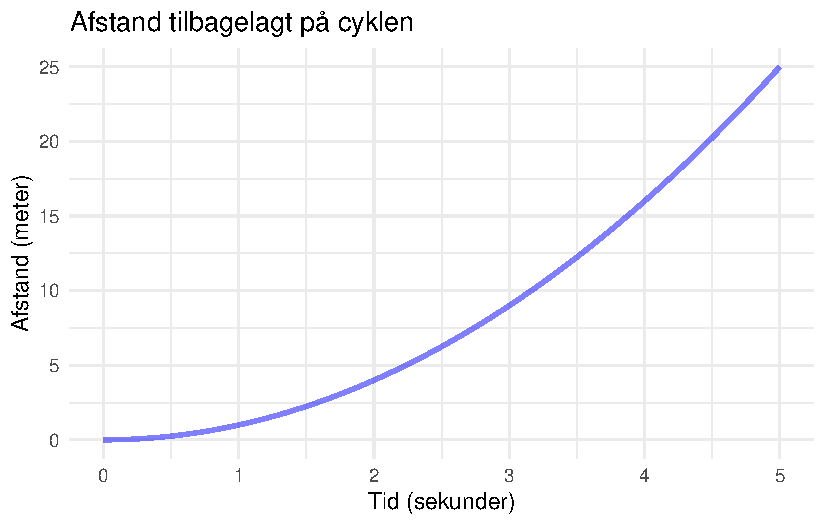
\includegraphics{differentialregning_files/figure-pdf/plot-funktion-1.pdf}

I det her eksempel viser grafen, at du cykler hurtigere og hurtigere. Jo
længere tid der går, jo stejlere er grafen, og jo hurtigere stiger
afstanden. Sådan kan det jo ikke blive ved med at gå i virkeligheden,
for til sidst ville man cykle hurtigere end bilerne. Men for
hyggematematikkens skyld, holder vi fast i eksemplet lidt endnu.

\section{2. Hvad er en tangent?}\label{hvad-er-en-tangent}

En \textbf{tangent} er en lige linje, der rører grafen et bestemt sted
og viser, hvor stejl grafen er lige der. For vores cykel betyder
tangentens \textbf{hældning} cyklens \textbf{hastighed} på det
tidspunkt.

Tænk på det sådan: Når kurven er meget stejl, ændrer afstanden sig
hurtigt, hvilket er det samme som at sige, at du kører hurtigt.
Tangenten fortæller os præcis, hvor hurtigt du kører på et givet
tidspunkt.

Lad os tegne en tangent til grafen, når \(x = 3\ sekunder\):

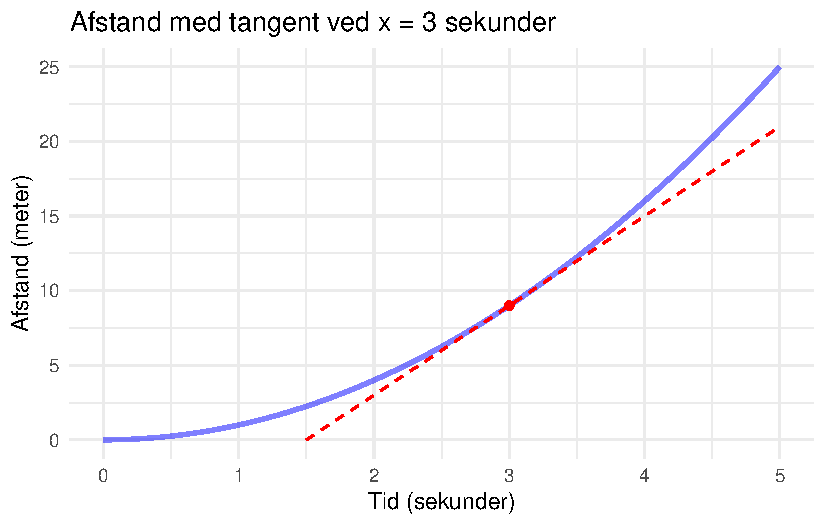
\includegraphics{differentialregning_files/figure-pdf/plot-tangent-1.pdf}

Den røde streg er tangenten ved \(x=3\). Hældningen af denne linje
fortæller os hastigheden, som vi snart finder ud af.

\section{3. Hvordan finder vi tangentens
hældning?}\label{hvordan-finder-vi-tangentens-huxe6ldning}

For at finde hastigheden (tangentens hældning), bruger vi
\textbf{differentiering}. Det betyder, at vi finder en ny regel, der
fortæller os, hvor stejl grafen er for hver tid \(x\).

Vores afstandsfunktion er:

\[ f(x) = x^2 \]

Når vi differentierer, får vi den \textbf{afledte} funktion, som er
hastigheden. Vi kalder den \(f'(x)\), som udtales ``f-mærke''.

\[ f'(x) = 2t \]

Lige nu skal du bare vide, at vi brugte en særlig regel, for at finde ud
af, at når \(f(x)=x^2\), så er \(f'(x) = 2x\). Den regel kommer vi
tilbage til.

Det vigtige lige nu er, at vi ved, at hastigheden ved
\(x = 3\ sekunder\) er:

\[ f'(3) = 2 \cdot 3 = 6 \text{ meter per sekund} \]

Så ved \(x=3\ sekunder\) kører du 6 meter per sekund. Den afledte
funktion \(f'(x)=2x\) giver os med andre ord hastigheden for enhver tid.

\section{4. Flere tangenter og deres
hældninger}\label{flere-tangenter-og-deres-huxe6ldninger}

Lad os tegne grafen igen, men nu med tangenter ved flere tidspunkter, så
vi kan se, hvordan hastigheden ændrer sig. Vi vælger \(x=1,2,3\):

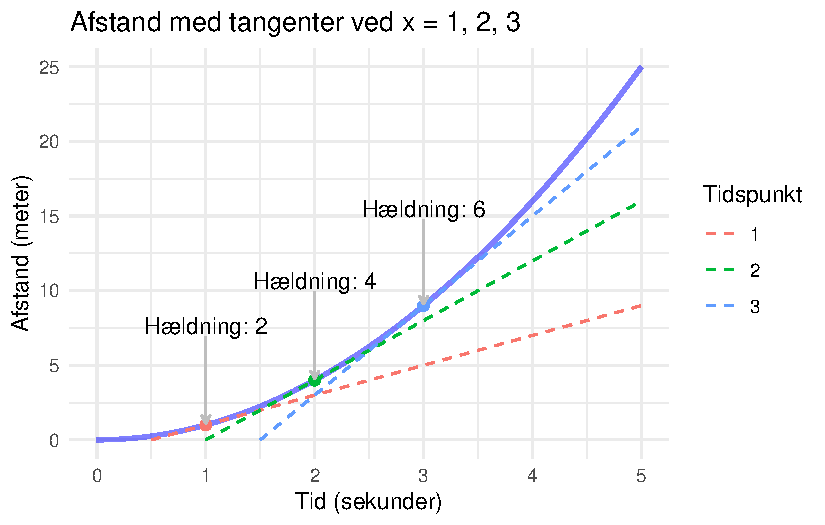
\includegraphics{differentialregning_files/figure-pdf/flere-tangenter-1.pdf}

Hver tangent viser hastigheden ved et bestemt tidspunkt: 1, 2, eller 3
sekunder. Bemærk, at hældningerne bliver større, når tiden stiger -- det
betyder, at cyklen kører hurtigere og hurtigere.

\section{5. Den afledte funktion:
Hastighedsgrafen}\label{den-afledte-funktion-hastighedsgrafen}

Den afledte funktion \(f'(x) = 2x\) er faktisk en graf over hastigheden.
Lad os tegne den for at se, hvordan hastigheden ændrer sig over tid:

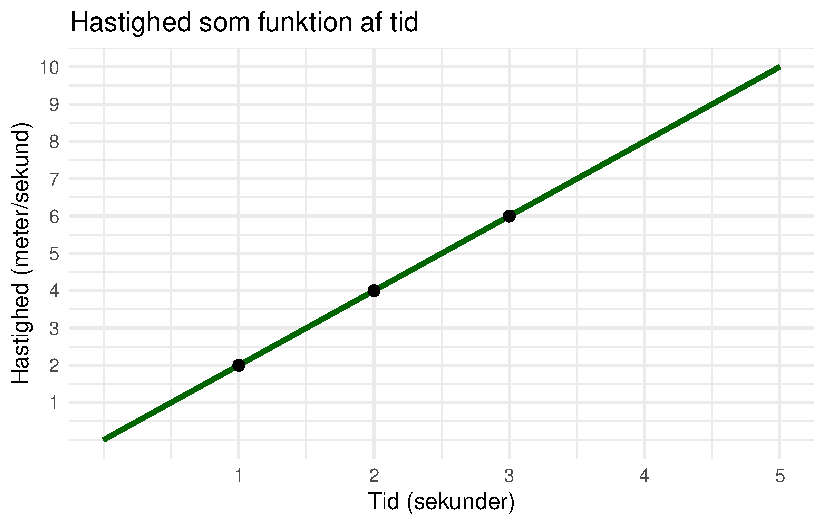
\includegraphics{differentialregning_files/figure-pdf/plot-afledte-1.pdf}

Grafen viser, at hastigheden stiger jævnt og følger en ret linje. Hvis
vi kigger tilbage på tangenterne, kan vi se, at hældningerne
(hastighederne) passer med værdierne på denne graf. For eksempel ved
\(x = 3\) er hastigheden 6, præcis som vi beregnede.

\section{6. Den dobbelte afledte:
Acceleration}\label{den-dobbelte-afledte-acceleration}

Nu tager vi det et skridt videre. Nogle gange ændrer hastigheden sig
mere og mere over tid -- det kalder vi \textbf{acceleration}. For at
finde accelerationen, differentierer vi hastighedsfunktionen (den
afledte) én gang til. Det kaldes den \textbf{dobbelt afledte}.

Hastighedsfunktionen er:

\[f'(x) = 2x\]

Når vi differentierer igen, får vi:

\[f''(x) = 2\]

Dette betyder, at accelerationen er 2 meter per sekund per sekund (eller
\(2 \text{m/s}^2\)). Det er konstant, så cyklen øger sin hastighed med 2
meter per sekund for hvert sekund.

\section{7. Illustration af
acceleration}\label{illustration-af-acceleration}

Lad os tegne en graf for accelerationen for at gøre det tydeligt:

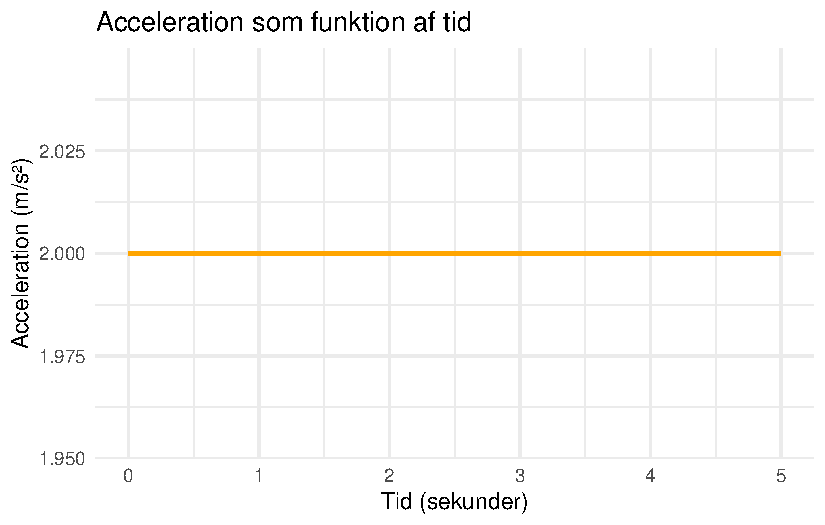
\includegraphics{differentialregning_files/figure-pdf/plot-acceleration-1.pdf}

Denne graf er en lige linje, fordi accelerationen er konstant. Det
fortæller os, at cyklen hele tiden får lige meget mere fart.

\section{8. Et knap så enkelt
eksempel}\label{et-knap-suxe5-enkelt-eksempel}

Lad os sige, at vi i stedet for vores første, ret enkle funktion,
\(f(x) = x^2\), bruger en mere kompliceret funktion, lad os kalde den
\(g(x)\):

\[ g(x) = x^3 - 18x^2 + 80x \] Her er \(x\) stadig tiden (i sekunder),
og \(g(x)\) er afstanden (i meter). Denne funktion er en
tredjegradsligning, hvilket betyder, at grafen ikke bare stiger eller
falder hele tiden -- den kan gå op og ned som en rutsjebane.

Lad os starte med at tegne grafen for at se, hvordan din cykeltur ser
ud:

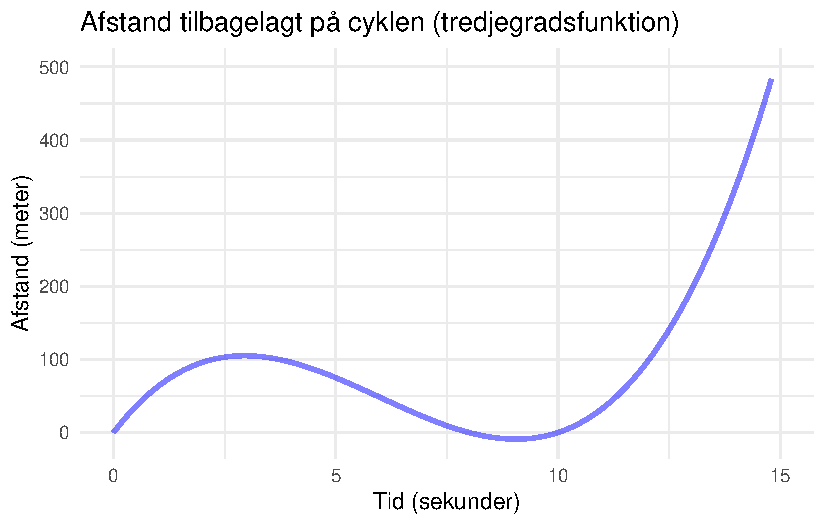
\includegraphics{differentialregning_files/figure-pdf/unnamed-chunk-1-1.pdf}

Som man kan se, stiger afstande de første par sekunder, men så
\emph{falder} den igen. Man kan forestille sig, at du havde glemt
cykelhjelmen, vendte om og hentede den, og så startede turen en gang
til. Til sidst, når du er kommet godt i gang, går det hurtigt fremad.

Ligesom før vil vi tegne tangenter for at finde hastigheden på
forskellige tidspunkter. Tangenten viser, hvor stejl grafen er, og det
fortæller os, hvor hurtigt du cykler. Vi vælger fem tidspunkter:
\(x=1, 2.5, 5, 10, 15\).

For at tegne tangenterne skal vi bruge den afledte funktion til at finde
hældningen. Den afledte af \[ g(x) = x^3 - 18x^2 + 80x \] er:

\[ g'(x) = 3x^2 - 36x + 80 \]

Den differentieringsregel vi bruger her, ser sådan ud:

\[ f(x) = x^n \] \[ f'(x) = nx^{(n-1)} \] (\emph{Hvorfor} den regel
gælder, kan du finde en forklaring på til allersidst.)

\(g'(x)\) er altså en funktion, der ortæller os hastigheden, eller
hændingen til tangenten, for hver tid, \(x\). For at tegne tangenten ved
en bestemt x-værdi, \(x_0\), bruger vi ligningen for tangentlinjen:
\[ y = g(x_0) + g'(x_0) \cdot (x - x_0) \] Lad os tegne grafen med nogle
tangenter, så vi får et indtryk af, hvordan det virker:

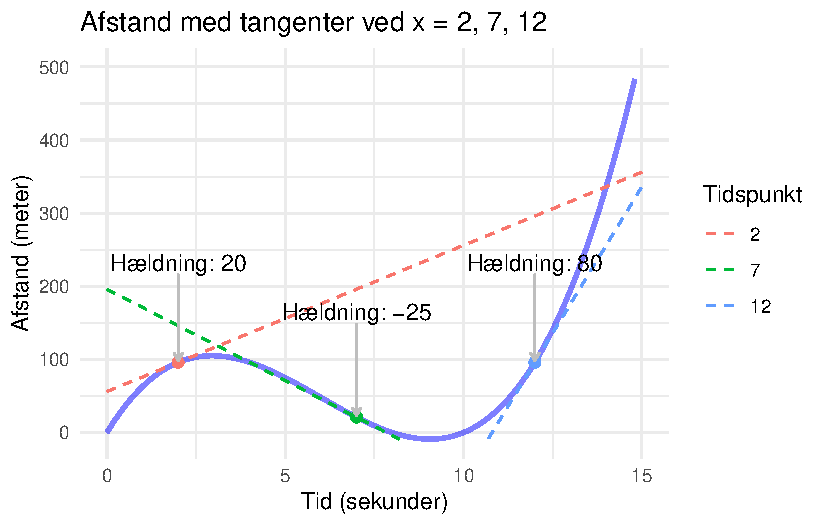
\includegraphics{differentialregning_files/figure-pdf/unnamed-chunk-2-1.pdf}

\section{Opsummering}\label{opsummering}

\begin{itemize}
\tightlist
\item
  Vi startede med at kigge på, hvor langt en cykel kører \(f(x) = x^2\).
\item
  Vi fandt ud af, at tangentens hældning viser \textbf{hastigheden}, og
  vi brugte differentiering til at finde hastighedsfunktionen
  \(f'(x) = 2x\).
\item
  Vi tegnede tangenter og så, at hastigheden stiger over tid.
\item
  Til sidst lærte vi om \textbf{acceleration} ved at differentiere igen
  \(f''(x) = 2\), og vi tegnede en graf for at vise, at accelerationen
  er konstant.
\end{itemize}

\bookmarksetup{startatroot}

\chapter{Enheder}\label{enheder}

\section{Hvad er enheder?}\label{hvad-er-enheder}

\bookmarksetup{startatroot}

\chapter{Logaritmer}\label{logaritmer}

\section{Hvad er logaritmer?}\label{hvad-er-logaritmer}



\end{document}
